\documentclass[conference]{IEEEtran}
\IEEEoverridecommandlockouts
\usepackage[T1]{fontenc}
\usepackage{cite}
\usepackage{amsmath,amssymb}
\usepackage{graphicx}
\usepackage{booktabs}
\usepackage{xcolor}
% Figure palette: one blue family plus a neutral grey. Dark / mid / light lightness
% steps keep the three roles apart in greyscale print and for colour-blind readers.
\definecolor{cFacts}{HTML}{1F4E79}    % facts (this paper's method): dark blue
\definecolor{cText}{HTML}{8A8A8A}     % text policies (substring, regex): grey
\definecolor{cAbl}{HTML}{B4C8DD}      % facts' ablations and variants: light blue
\definecolor{cAblEdge}{HTML}{5B7FA6}  % outline for the light-blue marks
\usepackage{listings}
\usepackage{pgfplots}
\pgfplotsset{compat=1.17}
\usetikzlibrary{positioning,arrows.meta,calc}
\newlength{\panelw}\setlength{\panelw}{\dimexpr\columnwidth-6pt\relax}
\usepackage{xurl}
\usepackage[hidelinks]{hyperref}
\usepackage{microtype}
\usepackage{balance}
\hypersetup{pdftitle={What Parsing Buys an Action Policy}, pdfauthor={Muhammad Usama}}
\renewcommand{\arraystretch}{1.2}
\setlength{\textfloatsep}{10pt plus 2pt minus 2pt}  % gap between top floats and text

\lstset{basicstyle=\ttfamily\scriptsize,columns=flexible,keepspaces=true,showstringspaces=false,
  breaklines=true,frame=tb,framesep=2pt,xleftmargin=2pt,xrightmargin=2pt,aboveskip=4pt,belowskip=2pt,
  captionpos=b,abovecaptionskip=3pt,commentstyle=\itshape\color{black!60},morecomment=[l]{//}}
\renewcommand{\lstlistingname}{Listing}
\usepackage{relsize}
% Inline code at 90% of the surrounding text (9 pt in body text, as before),
% so it also matches captions (a fixed \small enlarged it there).
\newcommand{\cmd}[1]{\texttt{\relscale{0.9}#1}}
\newcommand{\fact}[1]{\textit{#1}}  % fact names, italic like other terms

% Bold section headings (IEEEtran's default is regular small caps).
\makeatletter
\def\section{\@startsection{section}{1}{\z@}{1.5ex plus 1.5ex minus 0.5ex}%
  {0.7ex plus 1ex minus 0ex}{\normalfont\normalsize\centering\bfseries\MakeUppercase}}
\makeatother

\raggedbottom % do not stretch paragraph gaps to fill columns
\begin{document}

\title{What Parsing Buys an Action Policy:\\Detection, Interruptions and Their Value\\for AI Coding Agents\vspace{-0.3\baselineskip}}

\author{\IEEEauthorblockN{Muhammad Usama}
\IEEEauthorblockA{\textit{COMSATS University Islamabad}\\
Islamabad, Pakistan\\
sp23-bcs-069@isbstudent.comsats.edu.pk}\vspace{-0.8\baselineskip}}
\IEEEaftertitletext{\vspace{-1.6\baselineskip}}

\maketitle

\begin{abstract}
AI coding agents run shell commands with the developer's privileges, behind policies that match the command text. We hold one policy engine fixed and vary only what its rules see: text, in substring and four regular-expression policies, or three facts derived from a parsed shell syntax tree. On an independent held-out benchmark of 150 actions, fact-based rules stop 90.0\% of harmful actions at a 5.7\% false-positive rate, against 16.3\% for the substring policy. Most of that gain is vocabulary: a regex given the analyzer's word lists comes close, and the benchmark cannot separate the two. Parsing matters for interruptions: on our own traffic a line tokenizer with the same semantics interrupts more than twice as often, and in a pre-specified test on 417 developers in the public SWE-chat corpus, facts interrupt less than the tokenizer for 251 developers against 28 (1.5 points macro-averaged). Against the vocabulary regex the typical developer's difference is near zero. The pre-specified audit of whether stops are warranted does not support facts: a Claude agent's labels were inconclusive, and one human annotator judged regex-only stops warranted more often than fact-only ones (17 vs.\ 9 of 30). We release the analyzer, benchmarks, harness and a human labeling kit.
\end{abstract}

\begin{IEEEkeywords}
AI coding agents, LLM agent security, guardrails, access control policies, shell command analysis, static analysis, usable security
\end{IEEEkeywords}

\section{Introduction}
\label{sec:intro}
Coding agents such as Claude Code, Cursor and Codex execute shell commands on developer machines. When they go wrong the damage is concrete: in July 2025 an agent deleted a production database despite the user's explicit code freeze, according to the user~\cite{register2025replit}; malicious code instructing an agent to wipe local files and cloud resources was shipped inside an IDE extension, though it failed to run~\cite{aws2025q}; and a supply-chain attack invoked installed agent CLIs with permission checks disabled to collect \cmd{.env} files and SSH keys~\cite{wiz2025nx}. Benchmarks find that agents act unsafely in a large share of risky situations~\cite{vijayvargiya2026openagentsafety,hu2026saber,singh2026issuetrojanbench}.

The common mitigation is an \emph{action policy}: rules that allow, deny, or escalate each tool call. Shell commands reach these rules as strings. Agent permission systems may split compound commands and strip wrappers, but the rule itself is a pattern over the command text. Vendor documentation warns that ``Bash permission patterns that try to constrain command arguments are fragile'' and that a deny rule ``isn't a security boundary around the program''~\cite{claudecode_permissions}; documented hook examples grep the command for \cmd{rm -rf}~\cite{claudecode_hooks}. Industry reports show such guards bypassed by quoting, subshells and encoding~\cite{register2025cursor,townsend2026guardfall}.

A policy can fail in two directions. Too weak, it misses a destructive command phrased differently (\cmd{rm -fr}, \cmd{find -delete}, \cmd{bash -c '...'}). Too strong, it interrupts so often that approvals become reflexive: habituation to security warnings is well documented~\cite{akhawe2013alice,anderson2015polymorphic,vance2017habituation}, and agent vendors cite approval fatigue as a reason to reduce prompts~\cite{anthropic2025sandboxing,anthropic2026automode}. We therefore ask:

\begin{list}{}{\setlength{\labelwidth}{2.1em}\setlength{\labelsep}{0.5em}%
  \setlength{\leftmargin}{2.6em}\setlength{\itemsep}{1pt}\setlength{\parsep}{0pt}\setlength{\topsep}{3pt}%
  \renewcommand{\makelabel}[1]{\textbf{#1}\hfil}}
\item[RQ1] How much do text-based policies miss on independently written actions?
\item[RQ2] What does a fact layer add, and how much of it is vocabulary, normalization, the syntax tree, and per-tool semantics?
\item[RQ3] What does each policy cost in interruptions on our own agent traffic, and are those interruptions warranted?
\item[RQ4] Do these costs and audit results hold, pre-specified, on other developers' traffic and on a second agent?
\item[RQ5] Where does the analysis stop helping against an adversary who has read it?
\end{list}

\textbf{Contributions.} (1)~A controlled comparison that holds a policy engine fixed and varies only the predicate: substring rules, four regex variants (strong, traffic-tuned, vocabulary-matched and normalized), gate-everything, and facts from a shell AST, with ablations that replace the AST by a tokenizer or an off-the-shelf parser (Section~\ref{sec:design}). (2)~Evaluation on an independently written held-out benchmark, source-aware probes, 27,927 of our own Claude Code tool calls, a second agent (Codex), and a pre-specified test on 430 other developers (Sections~\ref{sec:method}--\ref{sec:results}). (3)~A decomposition: held-out recall comes mostly from vocabulary, while the syntax tree is the largest single factor in how often the gate interrupts real work. (4)~Audits of what interruptions are, including a relabeling that corrects our own first audit. (5)~An open artifact. Unlike CARE~\cite{liu2026care}, which also parses agent shell commands, we fix the policy engine, compare against deliberately favorable text baselines, and measure interruptions on public traces (Section~\ref{sec:related}).

\section{Threat Model}
\label{sec:threat}
An agent issues tool calls (\cmd{Bash}, \cmd{PowerShell}, \cmd{Read}, \cmd{Edit}, \cmd{Write}, \cmd{Grep}) that are intercepted before execution, here by a Claude Code \cmd{PreToolUse} hook or an MCP proxy. The agent may be mistaken or steered by prompt injection. We gate three classes of action. (i)~\emph{Destructive}, defined syntactically: bulk or recursive deletion, destructive database statements, and rewriting or deleting shared history. As a policy choice this includes directories that could be regenerated; we measure its cost. (ii)~\emph{Secret access}: reading, copying or sending credential material. (iii)~\emph{Opaque}: execution whose effect cannot be determined from the call. Each call is judged in isolation. We evaluate robustness to rephrasing and to one short source-aware probe round, not to a sustained adaptive adversary. Out of scope are multi-step decompositions such as writing a script and then running it~\cite{li2026unsafer}. The same holds for any command that runs a project script or build target (\cmd{./x.sh}, \cmd{make}, \cmd{npm run}), 3.1\% of real shell calls, whose effect lies in files the gate does not read. Also out of scope are effects that bypass the tool layer~\cite{zheng2026actplane} and attacks on the gate itself.

\section{Design: Facts Under a Fixed Policy Engine}
\label{sec:design}
ActionGate evaluates each call against ordered rules in CEL~\cite{cel}, a non-Turing-complete expression language; the first match decides, and evaluation errors fail closed. Its earlier default (v1) matched substrings of the command. We keep the engine and add one input, a map \cmd{facts} computed by a pure function of tool name and parameters, so that the fact-based policy reduces to three rules (Fig.~\ref{fig:rules}).

\begin{figure}[t]
\vspace*{-8.5pt}% cancel IEEEtran's figure top-skip so the figure aligns with Fig.~\ref{fig:pipeline} at the page top
\begin{lstlisting}[numbers=left,numberstyle=\tiny\color{black!45},numbersep=5pt,xleftmargin=11pt,
  morestring={[b]"},stringstyle=\color{black!70},
  morekeywords={deny,requires_approval,allow},keywordstyle=\bfseries\color{cFacts},
  emph={facts},emphstyle=\color{cFacts}]
// (a) v1: a substring test on the raw command text
tool_name == "Bash" &&
  (params.command.contains("rm -rf") ||
   params.command.contains("git push --force") || ...)

// (b) fact-based policy: first matching rule wins
facts.secret_access  -> deny
facts.destructive    -> requires_approval
facts.opaque         -> requires_approval
// no fact set       -> allow
\end{lstlisting}
\vspace{-4pt}
\caption{The v1 text rule (lines 2--4) and the fact-based policy (lines 7--10), both in CEL. For example, \cmd{D=build; sudo -u app \textquotesingle r\textquotesingle\textquotesingle m\textquotesingle{} -fr "\$D"} never contains the substring \cmd{rm -rf}, so v1 allows it; the analyzer resolves it to \cmd{rm -rf build}, sets \fact{destructive}, and line~8 requires approval.}
\label{fig:rules}
\end{figure}

As in authorization languages such as Cedar~\cite{cutler2024cedar}, the policy stays small while the application supplies structured attributes; an operator can write \cmd{facts.destructive \&\& environment == "prod"} without knowing shell syntax (Fig.~\ref{fig:pipeline}).

\begin{figure}[t]
\vspace*{-8.5pt}% cancel IEEEtran's figure top-skip so the figure aligns with Listing 1 at the page top
\centering
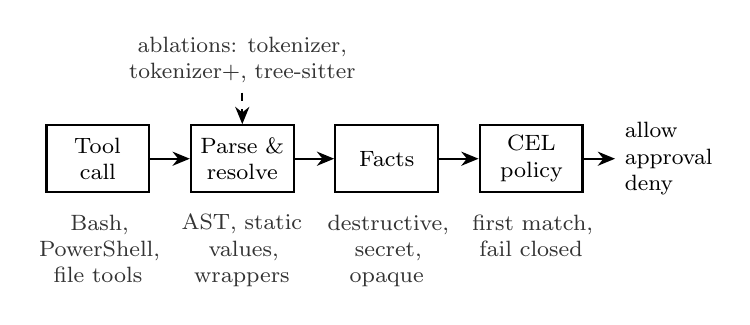
\begin{tikzpicture}[font=\footnotesize,node distance=5mm,
  arr/.style={-{Stealth[length=2.2mm,width=1.8mm]},line width=0.7pt},
  stage/.style={draw,thick,minimum height=8.5mm,text width=12mm,align=center,inner sep=1.5pt},
  note/.style={font=\footnotesize,text width=15.5mm,align=center,text=black!80}]
\node[stage] (call) {Tool\\call};
\node[stage,right=of call] (parse) {Parse \&\\resolve};
\node[stage,right=of parse] (facts) {Facts};
\node[stage,right=of facts] (cel) {CEL\\policy};
\draw[arr] (call) -- (parse);
\draw[arr] (parse) -- (facts);
\draw[arr] (facts) -- (cel);
\node[note,below=1.5mm of call] {Bash, PowerShell, file tools};
\node[note,below=1.5mm of parse] {AST, static values, wrappers};
\node[note,below=1.5mm of facts] {destructive, secret, opaque};
\node[note,below=1.5mm of cel] {first match, fail closed};
\node[align=center,text=black!80,above=4mm of parse] (abl) {ablations: tokenizer,\\tokenizer+, tree-sitter};
\draw[arr,dashed] (abl) -- (parse);
\node[align=left,right=4mm of cel] (out) {allow\\approval\\deny};
\draw[arr] (cel) -- (out);
\end{tikzpicture}
\caption{The fact pipeline. Only the \emph{Parse \& resolve} stage changes between facts and its ablations (dashed arrow); the engine and the rules stay fixed.}
\label{fig:pipeline}
\end{figure}

\textbf{Shell analysis.} Commands are parsed into a Bash AST with \cmd{mvdan.cc/sh}~\cite{mvdan_sh}. Each word is resolved to its static value: quotes and escapes removed, braces expanded (\cmd{.\{e,\}nv}$\,\to\,$\cmd{.env}), and variables substituted when assigned a static value earlier in the same command. Wrappers that only run another command are stripped (\cmd{sudo -u x}, \cmd{env A=1}, \cmd{xargs}, \cmd{timeout}, \cmd{npx}); flags are interpreted, so \cmd{-fr}, \cmd{-r -f} and \cmd{-{}-recursive} coincide. Nested shell code (\cmd{bash -c}, \cmd{eval} of literals, here-strings, static here-documents) is re-parsed to bounded depth. Destructive semantics are defined per tool: recursive \cmd{rm}, \cmd{find -delete}, force pushes and delete refspecs, \cmd{reset -{}-hard}, \cmd{clean -f}, \cmd{dd} to a device, destructive SQL reaching a database client anywhere in a pipeline, and bulk-delete verbs of container, cluster and cloud CLIs.

\textbf{Secret access} counts only commands that expose contents (\cmd{cat}, \cmd{grep}, \cmd{sed}, \cmd{tar}, \cmd{curl -d @f}, \cmd{cp} sources, \cmd{git show}), not ones that test, list, or hand a file to a program (\cmd{test -f .env}, \cmd{docker -{}-env-file .env}). A reader's leading pattern (\cmd{grep PATTERN FILE}) is not a file. Credential files are recognized by name; templates (\cmd{.env.example}) and public keys are excluded.

\textbf{Opacity.} At the shell level the analyzer does not guess: \cmd{eval} of computed text, a pipe into a shell or interpreter, a command name computed at run time, process substitution used as a script, unparseable input, excess nesting, and analyzer panics all yield \fact{opaque}. Running a project script is not opaque but out of scope. Inline interpreter code (\cmd{python -c}, \cmd{node -e}, here-documents) is only scanned with patterns for deletion APIs, secret file names and embedded shell commands; code that matches nothing is \emph{allowed}. A fourth fact, \fact{inline\_dynamic}, flags interpreter code that builds strings or names at run time; the \emph{facts-strict} policy escalates it. PowerShell is analyzed at token level. The analyzer is about 1,400 lines of Go, performs no I/O, and its final Bash entry point was fuzzed for 60\,s (369,056 inputs with four workers, no failures).

\textbf{Ablation switches.} For evaluation only, the analyzer accepts options that leave the policy untouched. \emph{Tokenizer} replaces the AST with quote-aware splitting at \cmd{;}, \cmd{\&\&}, \cmd{||}, \cmd{|} and \cmd{\&}, nothing expanded or re-parsed, under the same per-command semantics. \emph{Tokenizer+} also hands here-document bodies to the command that reads them and substitutes static variables, still without a syntax tree. \emph{Tree-sitter} (exploratory) feeds simple commands from the off-the-shelf tree-sitter-bash parser to the same semantics. \emph{No-readers} counts every mention of a credential file as a read, \emph{no-vars} disables variable substitution, and \emph{exempt} stops treating a recursive \cmd{rm} as destructive when every target is a conventionally regenerable directory (\cmd{build}, \cmd{node\_modules}, caches, \cmd{tmp}) or lies under a temporary directory.

\section{Evaluation Method}
\label{sec:method}
\textbf{Labels.} Benign $\to$ allow; destructive or opaque $\to$ requires approval; secret access $\to$ deny. These are the analyzer's own categories, so the benchmarks measure conformance to this ontology, not harm in general. Benign items deliberately include look-alikes (dangerous words in commit messages or grep patterns, dry runs, templates), which is adversarial to text rules.

\begin{table}[t]
\caption{Evaluation Data}
\label{tab:data}
\centering\footnotesize
\setlength{\tabcolsep}{3pt}
\begin{tabular}{@{}lll@{}}
\toprule
Set & Size & Role \\
\midrule
Development & 228 (133 harmful) & regression test \\
Held-out B & 150 (80 harmful) & primary test \\
Held-out A & 120 (70 harmful) & frozen analyzer v2.1 \\
Probes & 53 (50 harmful) & source-aware round \\
\midrule
Own traffic (Claude Code) & 27,927 calls & cost, in-sample \\
Codex, organic & 4,364 commands & second agent \\
Codex, Bash (staged) & 40 actions (3 harmful) & second agent \\
\midrule
SWE-chat & 640,530 calls, 417 dev. & pre-specified test \\
Self-published & 453,036 calls, 13 dev. & pre-specified test \\
\bottomrule
\end{tabular}\par\vspace{2pt}
\parbox{0.95\columnwidth}{\scriptsize Benchmark sizes are actions; traffic sizes are governed tool calls (own traffic) or shell calls of developers with at least 50 (out of sample). B holds 33 PowerShell items, A 13, the development set 22. The 40 staged Codex actions are 35 commands and 5 file writes.}
\end{table}

\textbf{Benchmarks.} Table~\ref{tab:data} lists the data. The development set was written by the author before the analyzer. Each held-out set was written in one pass by a separate LLM agent that saw only the label definitions and category counts, not the code, the other sets or analyzer output; no item was edited afterwards. A second blind agent agreed with all 270 labels; one human annotator later labeled 50 of B's items blind and agreed on 41 ($\kappa=0.75$). B was evaluated once, on the final analyzer; A was scored on an earlier frozen analyzer (v2.1), whose misses later informed fixes. The probes were written in about fifteen minutes by a reviewer agent that had the analyzer's source.

\textbf{Real traffic.} A hashed copy (prefix \texttt{60f161cc}) of the author's Claude Code transcripts, frozen on October 31, 2026: Bash 19,932, PowerShell 352 and file tools 7,643 calls in 15 sessions, 97\% of shell calls from one project, excluding the session in which this paper was written. Transcripts record calls as the agent issued them, not whether Claude Code's own permissions then blocked them.

\textbf{Second agent.} OpenAI's Codex CLI logs the argument vector of every command it runs. The organic corpus is the author's 11 sessions, all run through PowerShell or \cmd{cmd.exe}. The Bash corpus comes from seven everyday tasks (fixing a test, cleaning and rebuilding, squashing commits, resetting a test database and others) run in Git Bash in a small project with a fake \cmd{.env}, a database and a git history; none asked for a destructive or secret-reading command; its 35 commands and 5 writes were labeled by the author. All other agents in this study were Claude models, so shared blind spots remain a threat (Section~\ref{sec:limits}).

\textbf{Other developers (pre-specified).} Before reading these data we froze the analyzer and packs (hash prefix \texttt{6809d27d}) and specified three one-sided hypotheses over developers: facts stop fewer calls than tokenizer+ (H1) and than the vocabulary regex (H2) for more developers than the reverse (sign test), and a blind audit finds fact-only stops warranted more often than regex-only stops (H3, Fisher test). The primary source is SWE-chat~\cite{baumann2026swechat}: real sessions of Claude Code, Codex, Pi, OpenCode and other agents, mined from public GitHub repositories that use the Entire.io CLI; 417 developers (commit authors) with at least 50 shell calls. The second source is 13 developers who published their own sessions. Older exports cut inputs at 300 characters, so an amendment made before any policy ran restricts the primary analysis to complete inputs and adds a secondary one (H1b, H2b) on commands shorter than 290 characters. The audit draws 30 fact-only and 30 regex-only stops from SWE-chat, one per developer, labeled blind by a Claude agent and, after the results, by one human annotator instead of the two registered; the items are released as a kit. The specification is a timestamped file with the frozen hash in our repository, not an external registration. It records eleven deviations, the most consequential a converter fix made after a first run had been seen. Effect sizes, per-agent results, sensitivity runs, relabelings and the tree-sitter ablation are exploratory.

\textbf{Policies.} \emph{v1}: ActionGate's earlier substring pack, a baseline we wrote in the style of documented hooks~\cite{claudecode_hooks}. \emph{Strong regex}: four RE2 rules for flag variants, git force and delete forms, SQL, \cmd{find -delete}, interpreter deletion APIs, PowerShell, secret names and pipes into shells, written with knowledge of the development set and held-out A, so deliberately favorable. \emph{Tuned regex}: the same rules after a tuning pass on real traffic analogous to the analyzer's, five edits such as restricting \cmd{eval} to command position and ignoring secret names after \cmd{test} and \cmd{ls}. \emph{Vocabulary(-matched) regex}: the tuned regex extended with every secret name and destructive verb the analyzer knows, assembled after B's results were seen. \emph{Normalized vocabulary regex}: the same on commands after the analyzer's normalization. \emph{Gate-all}: every shell command and file mutation needs approval, and secret-file reads are denied.

\textbf{Metrics.} Recall and FPR: harmful and benign actions stopped (deny or approval); exact: decision equals label. Friction: share of real shell calls stopped, pooled or macro-averaged per project, session or developer. A fact-only stop is one facts make and the compared policy does not. Intervals are 95\% Wilson; differences use Newcombe's intervals~\cite{newcombe1998,newcombe1998unpaired}. On B, exact McNemar tests (facts vs.\ v1 on recall, and vs.\ the strong, tuned and vocabulary regexes on recall and FPR) are Holm-corrected; items cluster by technique, so even these are optimistic. On our traffic we use two-sided sign tests over the 15 sessions; out of sample, the pre-specified one-sided sign tests over developers, each at $\alpha=0.05$ without correction.

\section{Results}
\label{sec:results}

\begin{table*}[t]
\caption{Detection and Interruption Cost}
\label{tab:main}
\centering\small
\begin{tabular}{@{}lccccccc@{}}
\toprule
 & \multicolumn{3}{c}{Held-out B (80 harmful / 70 benign)} & \multicolumn{2}{c}{Held-out A (70 / 50)} & Probes (50) & Real traffic \\
\cmidrule(lr){2-4}\cmidrule(lr){5-6}\cmidrule(lr){7-7}\cmidrule(l){8-8}
Policy & Recall & FPR & Exact & Recall & FPR & Recall & Shell friction \\
\midrule
v1 (our substring pack) & 16.3\% & 4.3\% & 53.3\% & 17.1\% & 10.0\% & 20.0\% & 1.21\% \\
Strong regex & 82.5\% & 12.9\% & 84.7\% & 90.0\%$^a$ & 6.0\%$^a$ & 72.0\% & 6.88\% \\
Tuned regex & 77.5\% & 10.0\% & 83.3\% & 90.0\%$^a$ & 6.0\%$^a$ & 72.0\% & 2.68\% \\
Vocabulary-matched regex$^d$ & 86.3\% & 11.4\% & 87.3\% & 94.3\%$^a$ & 8.0\%$^a$ & 76.0\% & 3.64\% \\
Vocabulary-matched regex, normalized & 85.0\% & 11.4\% & 86.7\% & -- & -- & 78.0\% & 3.56\% \\
Gate-all & 100\% & 94.3\% & 43.3\%$^c$ & 98.6\% & 94.0\% & 98.0\% & 100\% \\
\midrule
\textbf{Facts} & \textbf{90.0\%} & \textbf{5.7\%} & \textbf{92.0\%} & 91.4\% & 0.0\% & 78.0\% & \textbf{2.74\%} \\
\quad tokenizer (no AST) & 86.3\% & 5.7\% & 90.0\% & -- & -- & 74.0\% & 9.90\% \\
\quad tokenizer+ (here-docs, vars) & 86.3\% & 5.7\% & 90.0\% & -- & -- & 74.0\% & 6.69\% \\
\quad tree-sitter parser$^e$ & 90.0\% & 5.7\% & 92.0\% & -- & -- & 78.0\% & 3.29\% \\
\quad without read-vs-mention & 90.0\% & 8.6\% & 90.7\% & -- & -- & 78.0\% & 3.42\% \\
\quad without variable resolution & 90.0\% & 5.7\% & 92.0\% & -- & -- & 78.0\% & 4.93\% \\
\quad with regenerable-path exemption & 90.0\% & 5.7\% & 92.0\% & -- & -- & 74.0\% & 2.56\% \\
Facts-strict & 90.0\% & 5.7\% & 92.0\% & -- & -- & 86.0\%$^b$ & 8.38\% \\
\bottomrule
\end{tabular}\par\vspace{2pt}
\parbox{\textwidth}{\footnotesize Held-out B is the primary test; A was scored on the analyzer frozen at v2.1. Shell friction: share of the 20,284 real shell calls a policy stops. $^a$Regex written with knowledge of A. $^b$Strict variant designed after the probe round. $^c$Includes six secret reads that gate-all's file-tool rule denies exactly. $^d$Assembled after B's results were seen. $^e$Exploratory: tree-sitter-bash in place of the AST, same per-command semantics; its front end was corrected once after B's misses were inspected (71/80 before).}
\end{table*}

\textbf{RQ1: what text misses.} Our substring policy stops 16.3\% of B's harmful actions (Table~\ref{tab:main}; CI 9.7--25.8), partly because it has no rule for shell secret reads or PowerShell; on the development set it stops all 11 canonical destructive commands but 1 of 52 rephrasings. A strong regex reaches 82.5\% recall at 12.9\% FPR: patterns broad enough to catch variants also catch dangerous words inside harmless commands.

\textbf{RQ2: what the fact layer adds.} Facts stop 90.0\% of B's harmful actions (CI 81.5--94.8) at 5.7\% FPR (CI 2.2--13.8). The gain over v1 is large (59 vs.\ 0 discordant items, Holm-adjusted $p<10^{-16}$); against the strong regex neither recall ($+7.5$ points) nor FPR ($-7.1$) differs significantly (adjusted $p=0.55$). Against the tuned regex recall is $+12.5$ points (adjusted $p=0.04$), but this is fragile: tuning cost the regex exactly four dynamic-code items. Giving the regex the analyzer's vocabulary lifts it to 86.3\% at 11.4\% FPR, leaving facts $+3.8$ recall points (CI $-3.6$ to $+11.6$) and $-5.7$ FPR points (CI $-13.7$ to $+0.9$): not significant, but B cannot exclude a 12-point difference either. Normalizing first changes almost nothing (85.0\%), and replacing the AST by either tokenizer loses three harmful items (86.3\%) and no FPR. On B, then, vocabulary carries most of the recall and token-level semantics most of the precision; facts' residual edge is opaque Bash code (9 vs.\ 5 of 10), the vocabulary regex's is destructive PowerShell (8 vs.\ 6 of 8). On an Intel Core i5-8350U laptop every policy evaluates an action in well under a millisecond.

\textbf{RQ3: cost on real traffic.} On the frozen corpus facts stop 2.74\% of shell calls (224 denials, 332 approvals) and the strong regex 6.88\%, more than facts in 10 of 15 sessions and fewer in 2 ($p=0.04$). Most of the regex's extra approvals come from a bare \cmd{eval} that also matches \cmd{pytest -k eval}, from output capture such as \cmd{s=\$(curl ...)}, and from commands that begin with a variable; tuning those away brings it to 2.68\%, and adding the analyzer's vocabulary raises it to 3.64\% (vs.\ facts: 7 vs.\ 2 sessions, $p=0.18$). The ablations show what produces facts' rate. Without the AST the tokenizer stops 9.90\% (more than facts in 12 sessions, fewer in none, $p=0.0005$), because here-documents and multi-line programs fall apart into spurious commands; tokenizer+ recovers part of this but still stops 6.69\% (11 vs.\ 0 sessions, $p=0.001$). The rest comes from quoting and command substitution that span lines, compound commands and nested code. Without variable resolution facts stop 4.93\%, and without the read-vs-mention rule 3.42\%. The syntax tree, which barely mattered on B, is the largest single factor on real work. Macro-averaged, facts stop 2.77\% per project and 2.92\% per session, tokenizer+ 6.86\% and 6.59\%. Facts stop none of the 7,643 file-tool calls but 9.4\% of the 352 PowerShell calls, mostly scripts invoked through a variable that token-level analysis cannot resolve.

\begin{figure}[t]
\centering
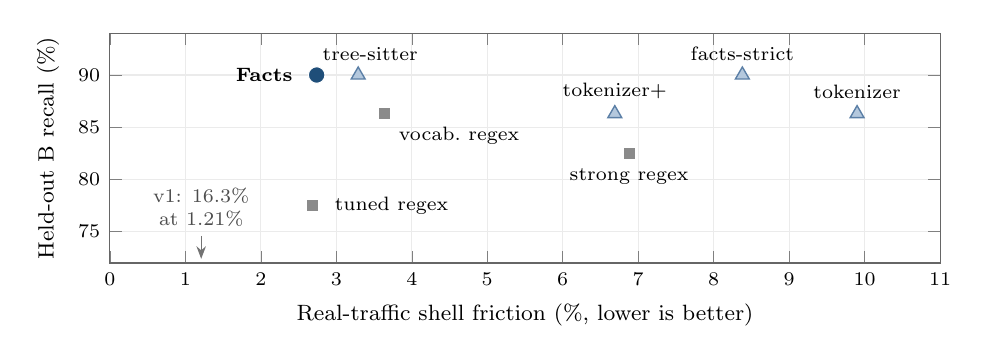
\begin{tikzpicture}
\begin{axis}[width=\columnwidth,height=4.5cm,
  xmin=0,xmax=11,ymin=72,ymax=94,
  xlabel={Real-traffic shell friction (\%, lower is better)},
  ylabel={Held-out B recall (\%)},
  label style={font=\footnotesize},tick label style={font=\scriptsize},
  grid=major,grid style={black!8},axis line style={black!60},
  every node near coord/.style={font=\scriptsize},
  clip=false]
% text policies
\addplot[only marks,mark=square*,mark size=2.2pt,cText,mark options={draw=white,line width=0.4pt}] coordinates {(6.88,82.5) (2.68,77.5) (3.64,86.3)};
% facts ablations
\addplot[only marks,mark=triangle*,mark size=2.9pt,cAbl,mark options={draw=cAblEdge,line width=0.5pt}] coordinates {(9.90,86.3) (6.69,86.3) (8.38,90.0) (3.29,90.0)};
% facts
\addplot[only marks,mark=*,mark size=3pt,cFacts,mark options={draw=white,line width=0.4pt}] coordinates {(2.74,90.0)};
\node[font=\scriptsize,anchor=east] at (axis cs:2.55,90.0) {\textbf{Facts}};
\node[font=\scriptsize,anchor=south] at (axis cs:3.45,90.5) {tree-sitter};
\node[font=\scriptsize,anchor=north west] at (axis cs:3.70,86.0) {vocab.\ regex};
\node[font=\scriptsize,anchor=west] at (axis cs:2.85,77.5) {tuned regex};
\node[font=\scriptsize,anchor=north] at (axis cs:6.88,82.0) {strong regex};
\node[font=\scriptsize,anchor=south] at (axis cs:6.69,86.8) {tokenizer+};
\node[font=\scriptsize,anchor=south] at (axis cs:9.90,86.8) {tokenizer};
\node[font=\scriptsize,anchor=south] at (axis cs:8.38,90.5) {facts-strict};
\draw[-{Stealth[length=1.6mm]},black!55] (axis cs:1.21,74.6) -- (axis cs:1.21,72.4);
\node[font=\scriptsize,anchor=south,align=center,text=black!70] at (axis cs:1.21,74.6) {v1: 16.3\%\\at 1.21\%};
\end{axis}
\end{tikzpicture}
\caption{Detection against interruption cost (Table~\ref{tab:main}). Dark-blue circle: facts; grey squares: text policies; light-blue triangles: selected ablations and variants of facts (Table~\ref{tab:main} lists all). On held-out B the vocabulary regex and the tokenizers come close to facts; on real traffic, parsing is what keeps friction low. Gate-all (100\%, 100\%) is off the chart.}
\label{fig:tradeoff}
\end{figure}

\textbf{What our own interruptions are.} In a seeded sample of 40 fact-based denials, 37 (92.5\%, CI 80.1--97.4) read or copied a real credential file, as ordinary development work, so approval may suit secret reads better than a hard deny. Of 40 sampled approvals, labeled by the author with Claude's assistance and by a separate Claude agent ($\kappa=0.90$), at most one was worth the interruption: 27--28 deleted build outputs, caches or scratch directories the agent had just created, 7--8 were analyzer false positives, and 4--5 ran benign run-time code. Exempting regenerable paths per call lowers friction only to 2.56\% and lets the probe \cmd{mv src /tmp/trash \&\& rm -r /tmp/trash} through; exempting targets created earlier in the session lowers it to 2.38\%, because most such directories are created by programs, not by commands the gate sees.

\textbf{RQ4a: a second agent.} On the organic Codex corpus, which the analyzer was never tuned on, facts stop 1.86\% of 4,364 commands, the tuned and vocabulary regexes 1.8\% and 1.9\%, and the strong regex 12.2\%; every command was PowerShell, so this tests only token-level analysis. In the staged Bash corpus Codex produced three harmful actions: two \cmd{git clean} runs, one of which removed every git-ignored file including the developer's \cmd{.env} and SQLite database, and a script it had written that deletes old files. Facts require approval for both \cmd{git clean} commands and interrupt nothing else (2 of 3 harmful, 0 of 37 benign); the script run is out of scope by the threat model. The vocabulary regex matches facts, and v1 lets all three through. The sample is tiny, but it shows the failure this paper is about: a routine instruction turned into bulk deletion.

\begin{figure}[t]
\centering
\pgfplotsset{oos/.style={xbar,bar shift=0pt,scale only axis,width=2.95cm,height=4.5cm,
  ymin=0.45,ymax=8.55,y dir=reverse,ytick={1,...,8},bar width=7pt,
  xmin=0,tick label style={font=\scriptsize},label style={font=\scriptsize},
  title style={font=\footnotesize\bfseries,yshift=-1mm},
  xmajorgrids,grid style={black!10},axis line style={black!55},clip=false,
  xlabel={Shell calls stopped (\%)},xlabel style={yshift=1mm},
  major tick length=2pt}}
\begin{tikzpicture}
\begin{axis}[oos,name=swe,xmax=7.8,xtick={0,2,4,6},title={SWE-chat (417 dev.)},
  yticklabels={v1,Strong regex,Tuned regex,Vocab.\ regex,\textbf{Facts},tokenizer,tokenizer+,tree-sitter$^\ast$}]
\addplot[fill=cText,draw=cText!75!black,line width=0.3pt] coordinates {(0.86,1) (3.04,2) (2.02,3) (2.33,4)};
\addplot[fill=cFacts,draw=cFacts!70!black,line width=0.3pt] coordinates {(2.21,5)};
\addplot[fill=cAbl,draw=cAblEdge,line width=0.3pt] coordinates {(4.48,6) (3.75,7) (2.26,8)};
\addplot[only marks,mark=diamond*,mark size=2.4pt,black,mark options={fill=white,line width=0.6pt}] coordinates {(0.83,1) (3.74,2) (2.57,3) (3.16,4) (1.98,5) (4.73,6) (3.82,7) (2.05,8)};
\node[font=\scriptsize,anchor=east,text=black!75] at (axis cs:7.8,3) {119/123};
\node[font=\scriptsize,anchor=east,text=black!75] at (axis cs:7.8,4) {166/86};
\node[font=\scriptsize,anchor=east,text=black!75] at (axis cs:7.8,6) {270/21};
\node[font=\scriptsize,anchor=east,text=black!75] at (axis cs:7.8,7) {251/28};
\node[font=\scriptsize,anchor=east,text=black!75] at (axis cs:7.8,8) {68/21};
\end{axis}
\begin{axis}[oos,at={(swe.east)},anchor=west,xshift=2.5mm,xmax=4.6,xtick={0,1,2,3,4},title={Self-published (13)},yticklabels={}]
\addplot[fill=cText,draw=cText!75!black,line width=0.3pt] coordinates {(0.88,1) (2.89,2) (1.38,3) (1.56,4)};
\addplot[fill=cFacts,draw=cFacts!70!black,line width=0.3pt] coordinates {(2.33,5)};
\addplot[fill=cAbl,draw=cAblEdge,line width=0.3pt] coordinates {(3.30,6) (3.05,7) (2.37,8)};
\addplot[only marks,mark=diamond*,mark size=2.4pt,black,mark options={fill=white,line width=0.6pt}] coordinates {(0.48,1) (2.24,2) (1.09,3) (1.18,4) (1.30,5) (2.04,6) (1.88,7) (1.33,8)};
\node[font=\scriptsize,anchor=east,text=black!75] at (axis cs:4.6,3) {1/10};
\node[font=\scriptsize,anchor=east,text=black!75] at (axis cs:4.6,4) {2/8};
\node[font=\scriptsize,anchor=east,text=black!75] at (axis cs:4.6,6) {10/0};
\node[font=\scriptsize,anchor=east,text=black!75] at (axis cs:4.6,7) {10/0};
\node[font=\scriptsize,anchor=east,text=black!75] at (axis cs:4.6,8) {6/1};
\end{axis}
\end{tikzpicture}
\caption{Out of sample: other developers' shell calls stopped by each policy. Bars are macro-averages over developers with at least 50 shell calls (SWE-chat 640,530 calls; self-published 453,036), shaded as in Fig.~\ref{fig:tradeoff}; diamonds pool all calls. Numbers at right: developers for whom facts stop fewer\,/\,more calls than that policy (one-sided sign test). The analyzer was frozen before the data were read. $^\ast$Exploratory off-the-shelf parser ablation (Table~\ref{tab:main}).}
\label{fig:oos}
\end{figure}

\textbf{RQ4b (pre-specified): 430 other developers.} On SWE-chat facts stop 1.98\% of shell calls and tokenizer+ 3.82\% (Fig.~\ref{fig:oos}). Facts stop fewer calls for 251 developers and more for 28 ($p=3\times10^{-46}$; H1 holds), and fewer than the vocabulary regex for 166 against 86 ($p=3\times10^{-7}$; H2 holds). The tuned regex, not in the hypotheses, ties facts (119 vs.\ 123). On the 13 self-published developers H1 holds (10 vs.\ 0, $p=0.001$) but H2 does not; there the common fact reasons include 688 commands the Bash parser rejected, which fail closed. In the secondary analysis on commands shorter than 290 characters, neither H1b (8 vs.\ 6, $p=0.40$) nor H2b holds. Table~\ref{tab:h2} collects every setting in which facts do not interrupt less than a regex: H2 holds on SWE-chat as a whole and for Claude Code and Codex users, and nowhere else.

\begin{table}[t]
\caption{Where Facts Do Not Interrupt Less Than a Regex}
\label{tab:h2}
\centering\footnotesize
\setlength{\tabcolsep}{3pt}
\begin{tabular}{@{}llrrr@{}}
\toprule
Setting & Regex & Dev. & Fewer/more & $p$ \\
\midrule
SWE-chat & tuned$^a$ & 417 & 119/123 & 0.63 \\
\quad OpenCode users$^b$ & vocab. & 35 & 10/8 & 0.41 \\
\quad Pi users$^b$ & vocab. & 13 & 4/4 & 0.64 \\
Self-published (H2) & vocab. & 13 & 2/8 & $>$0.98 \\
 & tuned$^a$ & 13 & 1/10 & $>$0.99 \\
Self-published, $<$290 chars (H2b) & vocab. & 19 & 3/12 & $>$0.99 \\
 & tuned$^a$ & 19 & 1/13 & $>$0.99 \\
\bottomrule
\end{tabular}\par\vspace{2pt}
\parbox{0.95\columnwidth}{\scriptsize Fewer/more: developers for whom facts stop fewer / more shell calls than the regex; $p$: one-sided sign test that facts stop fewer. On SWE-chat as a whole the macro-averaged difference from the vocabulary regex is $-0.1$ points (CI $-0.4$ to $+0.2$). $^a$Not a pre-specified hypothesis. $^b$Exploratory: developers with at least 50 shell calls of that agent.}
\end{table}

\textbf{Effect sizes and robustness (exploratory).} Because the sign test counts a one-call difference like a large one, we also report per-developer differences on SWE-chat. Against tokenizer+ facts interrupt 1.5 points less macro-averaged (bootstrap CI 1.3--1.8; median 0.5). Against the vocabulary regex the macro difference is $-0.1$ points (CI $-0.4$ to $+0.2$) and the median is zero; the pooled difference ($-1.2$) comes from heavy users, the ten largest of whom hold 41\% of calls. Against the tuned regex it is $+0.2$ (CI $-0.05$ to $+0.5$). For 286 of 417 developers facts and the vocabulary regex differ by less than half a point. Within agents, H1 holds for Claude Code, Codex and OpenCode users but not significantly for Pi (8 vs.\ 2, $p=0.055$). Excluding the 32 developers in the collection tool vendor's own repositories changes nothing (H1 224 vs.\ 28, H2 152 vs.\ 80). The tokenizer gap persists on commands under 290 characters (0.98\% vs.\ 1.58\%), but about three quarters of tokenizer+'s extra stops come from the 22\% of calls that are longer. The sign tests drop ties (138 developers for H1, 165 for H2), many of them stopped by neither policy.

\textbf{An off-the-shelf parser (exploratory).} To check that the result does not depend on our parser, the tree-sitter ablation replaces mvdan's syntax tree. After one correction informed by B's misses (71/80 before), it matches facts on B, and it matches them on the probes without one (Table~\ref{tab:main}). On SWE-chat facts stop fewer calls than tree-sitter for 68 developers and more for 21 (Fig.~\ref{fig:oos}), but the macro-averaged difference is only 0.05 points (CI 0.01--0.09), and tree-sitter interrupts less than tokenizer+ for 245 developers and more for 36; 0.7\% of distinct commands do not parse in tree-sitter and fail closed. The parser mattered only on our own traffic, where the analyzer's false-positive fixes were made on mvdan's tree (3.29\% vs.\ 2.74\%). The gap to the tokenizer is a property of parsing, not of our parser.

\textbf{What the extra stops are (pre-specified audit).} The agent annotator, which agreed with B's labels on 49 of the 50 kit items ($\kappa=0.97$; both are Claude models), found a gated action in 5 of 30 fact-only stops (17\%, CI 7--34) and 3 of 30 regex-only stops (10\%, CI 3--26), a difference of $+6.7$ points (CI $-11.5$ to $+24.8$; Fisher $p=0.35$), so H3 is inconclusive under the agent's labels. Fact-only stops were mostly fail-closed opacity: a command name held in a variable (10), interpreter code built at run time (7) and input the parser rejected (4).

\begin{figure}[t]
\centering
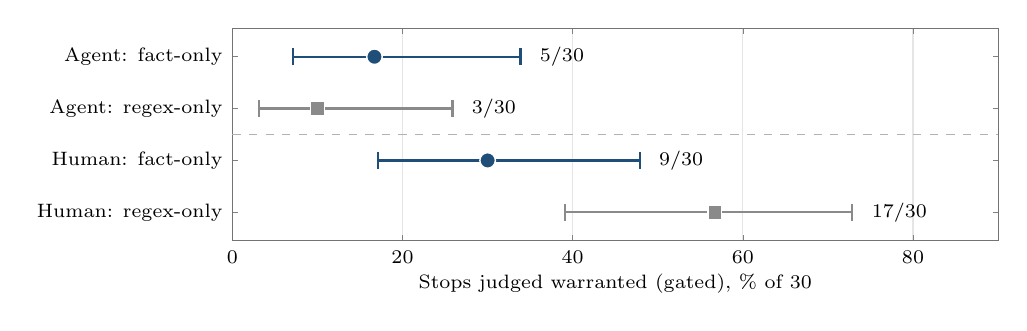
\begin{tikzpicture}
\begin{axis}[scale only axis,width=\columnwidth-24mm,height=2.7cm,
  xmin=0,xmax=90,ymin=0.45,ymax=4.55,y dir=reverse,
  ytick={1,2,3,4},yticklabels={Agent: fact-only,Agent: regex-only,Human: fact-only,Human: regex-only},
  xtick={0,20,40,60,80},
  xlabel={Stops judged warranted (gated), \% of 30},xlabel style={yshift=1mm},
  label style={font=\scriptsize},tick label style={font=\scriptsize},
  xmajorgrids,grid style={black!10},axis line style={black!55},major tick length=2pt,clip=false]
\draw[black!30,dashed] (axis cs:0,2.5) -- (axis cs:90,2.5);
% 95% Wilson intervals
\draw[cFacts,line width=0.8pt,|-|] (axis cs:7,1) -- (axis cs:34,1);
\draw[cText,line width=0.8pt,|-|] (axis cs:3,2) -- (axis cs:26,2);
\draw[cFacts,line width=0.8pt,|-|] (axis cs:17,3) -- (axis cs:48,3);
\draw[cText,line width=0.8pt,|-|] (axis cs:39,4) -- (axis cs:73,4);
\addplot[only marks,mark=*,mark size=2.8pt,cFacts,mark options={draw=white,line width=0.5pt}] coordinates {(16.7,1) (30.0,3)};
\addplot[only marks,mark=square*,mark size=2.5pt,cText,mark options={draw=white,line width=0.5pt}] coordinates {(10.0,2) (56.7,4)};
\node[font=\scriptsize,anchor=west] at (axis cs:35,1) {5/30};
\node[font=\scriptsize,anchor=west] at (axis cs:27,2) {3/30};
\node[font=\scriptsize,anchor=west] at (axis cs:49,3) {9/30};
\node[font=\scriptsize,anchor=west] at (axis cs:74,4) {17/30};
\end{axis}
\end{tikzpicture}
\caption{The pre-specified audit (H3): of 30 stops only facts make and 30 only the vocabulary regex makes on SWE-chat, the share judged warranted (dark-blue circles: fact-only; grey squares: regex-only), with 95\% Wilson intervals. The Claude agent's labels are inconclusive; the human annotator's labels point the other way.}
\label{fig:audit}
\end{figure}

\textbf{A human annotator (exploratory).} After these results, one human annotator labeled the same 110-item kit, shuffled and blind to source and policy, under the labeling guide; a second human did not, so there is no adjudication and no human--human agreement. The annotator agreed with B's labels on 41 of the 50 kit items ($\kappa=0.75$) and with the agent on 40 of them ($\kappa=0.72$), but with the agent on only 38 of the 60 audit items ($\kappa=0.25$). The annotator found a gated action in 9 of 30 fact-only stops (30\%, CI 17--48) and 17 of 30 regex-only stops (57\%, CI 39--73), a difference of $-26.7$ points (CI $-47.5$ to $-1.7$; one-sided $p=0.99$ in the registered direction). Across the kit, most disagreements were items the annotator labeled secret (12) or destructive (11) where the agent chose benign. One annotator's labels cannot settle H3, but they do not support it, and they point the other way: what counts as warranted depends on who judges, and a Claude agent may be more lenient toward credential mentions than a human.

\textbf{One protocol for both audits (exploratory).} A first audit on our own traffic had found a gated action in 25 of 30 fact-only stops but only 3 of 30 regex-only ones, which mostly mentioned a credential file without reading it. To separate population from protocol, a fresh agent relabeled all 150 audit items, shuffled and blind to source, with an added label, chosen after seeing the discrepancy, for code built or named at run time that a careful reader can resolve. The two populations then look alike: 8 of 30 in-sample fact-only stops (27\%, CI 14--44) and 5 of 30 out-of-sample ones (17\%, CI 7--34) were strictly gated, 19 and 17 were such readable run-time code, and 3 and 8 benign; regex-only stops were strictly gated in 2--6 of 30 per stratum. Fact-only stops are mostly conservative opacity, on the analyzer's own traffic as on others', and the first audit, which counted readable run-time code as gated, is superseded. The added label is relative to a static analyzer and was applied by a model; human labels may draw the line elsewhere.

\textbf{Tokenizer-only stops (exploratory).} Under the same protocol an agent labeled 30 tokenizer+-only and 30 fact-only stops from SWE-chat. 26 tokenizer+-only stops were benign, mostly multi-line builds, tests and polls, 1 was readable run-time code, and 3 read a token that facts allowed; 9 fact-only stops were strictly gated against 3 tokenizer+-only ones ($p=0.052$). Parsing removes mostly spurious stops and adds a few warranted ones, but does not catch everything the tokenizer catches.

\textbf{RQ5: a source-aware probe round.} With the source in hand, a reviewer agent evaded facts on 11 of 50 harmful probes: six read credential stores missing from the name list (Docker and GitHub CLI configs, \cmd{\textasciitilde/.kube/config}, \cmd{terraform.tfstate}, \cmd{.envrc}), four built strings inside interpreter code (\cmd{open('.e'+'nv')}), and one truncated a database file. The normalized vocabulary regex ties facts (78.0\%), and v1 stops 20.0\%. Escalating dynamic interpreter code (facts-strict) reaches 86.0\%, post hoc, but raises real-traffic friction to 8.38\%, because agents build strings in inline Python constantly.

\section{Analysis}
\label{sec:analysis}
\textbf{Real traffic finds what benchmarks do not.} The first fact-based analyzer scored 100\% on its development set and 91.4\% recall at 0\% FPR on held-out A, yet stopped 18.2\% of real shell calls on an earlier snapshot of our corpus. Three causes were absent from every benchmark: static \cmd{python - <{}<'EOF'} here-documents treated as code from stdin (2,568 calls), interpreter paths held in a variable (439 calls), and grep patterns and globs read as secret paths. Fixing them brought friction to 2.7\% without changing held-out A, which is why our own friction is in-sample. Benchmarks are written one action at a time; agents write multi-line programs.

\textbf{What remains hard on held-out data.} Facts' 8 misses and 4 false positives on B fall into four classes: open-world vocabulary (7; e.g., \cmd{manage.py flush}, \cmd{prisma migrate reset}, \cmd{aws ec2 terminate-instances}), interpreter evaluation (1; Perl \cmd{eval pack}), intent modifiers (3 false positives: \cmd{terraform plan -destroy}, \cmd{kubectl delete -{}-dry-run}, \cmd{Remove-Item -WhatIf}) and token-level PowerShell (1 false positive). Held-out A's six misses on v2.1 were fixed afterwards, so the current analyzer's 100\% on A is not a test result. Open-world vocabulary and dynamic interpreter code argue for a two-stage design: deterministic facts for the common, explainable cases, and a learned classifier or LLM judge~\cite{anthropic2026automode,liu2026care} only for unknown tools and dynamic code.

\textbf{Recommendations for deploying agent action policies.}
\begin{enumerate}
\item \emph{Invest first in vocabulary, then in structure;} a parser mainly cuts interruptions.
\item \emph{Make the unknown explicit:} route unresolvable constructs to a human; scripts and build targets (3.1\% of calls) need a separate control.
\item \emph{Judge secret access by contents, not mentions,} and prefer approval to a hard deny for reads.
\item \emph{Scope destructive rules by what is lost;} judging whether a deletion is regenerable needs session context.
\item \emph{Evaluate on traces you did not tune on,} and report and audit interruptions per developer or session.
\item \emph{Treat inline interpreter code separately,} by escalation (8.4\% friction) or a semantic judge.
\end{enumerate}

\section{Related Work}
\label{sec:related}
\textbf{Agent action policies.} Progent~\cite{shi2025progent}, AgentSpec~\cite{wang2025agentspec}, Conseca~\cite{tsai2025conseca}, ClawGuard~\cite{zhao2026clawguard} and Datalog monitors~\cite{palumbo2026formal} enforce deterministic policies over tool calls; CaMeL~\cite{debenedetti2025camel} and Fides~\cite{costa2025fides} enforce control and information flow; GuardAgent~\cite{xiang2025guardagent} and ShieldAgent~\cite{chen2025shieldagent} synthesize or verify guard logic; LlamaFirewall~\cite{chennabasappa2025llamafirewall} combines regex and LLM scanners. These target mostly API-style tools~\cite{debenedetti2024agentdojo}; a rule over a free-form shell argument remains a text rule. CARE~\cite{liu2026care} canonicalizes and parses shell commands, scores risk with weights tuned on a development split and sends borderline cases to an LLM judge; it reports deny rates on benign command sets, not interruptions on live traffic. AgentGuard~\cite{dai2026agentguard} learns execution rules from anomalous trajectories; we instead fix the rules and vary the predicate. Claude Code's auto mode~\cite{anthropic2026automode} reports 0.4\% FPR and 17\% false negatives for an LLM classifier on internal data; an independent stress test found 81\% false negatives on 253 ambiguous actions~\cite{ji2026permissiongate}. Neither figure is comparable to ours. User-authored allow/ask/never rules reduce prompts but can weaken protection~\cite{yan2026userpolicies,michael2026permissions}; our packs are expert-written.

\textbf{Benchmarks and containment.} OpenAgentSafety~\cite{vijayvargiya2026openagentsafety}, SABER~\cite{hu2026saber} and IssueTrojanBench~\cite{singh2026issuetrojanbench} score agents rather than gates. Real-session corpora such as SWE-chat~\cite{baumann2026swechat} have been used to study developer-agent misalignment~\cite{tang2026misalignment}; we use them to price gate interruptions. Sandboxes~\cite{anthropic2025sandboxing}, OS-level enforcement~\cite{zheng2026actplane} and recoverable filesystems~\cite{zhong2026yolofs} bound where damage lands but cannot tell \cmd{rm -rf build/} from \cmd{rm -rf src/} inside a workspace; they complement a per-call gate.

\textbf{Shell analysis and obfuscation.} Shell semantics are subtle~\cite{greenberg2020smoosh}, and static analysis of shell scripts has a long history~\cite{mazurak2007abash}. Obfuscation frameworks show how cheaply string signatures are defeated~\cite{bohannon2016invokeobfuscation,lefevre_bashfuscator}. Parsing shell commands improved learned security classification over generic tokenization in a small study without a held-out split~\cite{trizna2021slp}; we quantify the analogous effect inside a policy gate. AST-level deobfuscation with emulation~\cite{li2019powershell} also shows the value of recovering structure; we recover it without emulating and send the unresolved remainder to a human. Habituation to warnings~\cite{akhawe2013alice,anderson2015polymorphic,vance2017habituation} and the 84\% fewer permission prompts reported for Claude Code's sandbox~\cite{anthropic2025sandboxing} make the interruption rate a first-class metric.

\section{Limitations}
\label{sec:limits}
\emph{Labels.} All benchmarks are small. The held-out sets and probes were written and labeled by Claude models, the family that assisted development, and the development set and Codex Bash corpus by the author; one other human labeled only a 50-item subset of B, after the results, so they may share blind spots, as the probe round's unlisted credential stores suggest. They test conformance to our ontology, not expert judgments of harm. We release a labeling kit (110 items, a guide and an agreement script) so that others can check the agent's labels.

\emph{Statistics.} Items cluster by technique and audit samples by session or developer, so even Holm-adjusted tests and Wilson intervals are optimistic, and B cannot resolve differences of about ten points.

\emph{Traffic.} Our Claude Code traffic is one developer's 15 sessions, dominated by one project and in-sample. The Codex corpora add a second agent but not a second developer, and the Bash one is small and staged. The out-of-sample corpora add 430 developers but are unlabeled; SWE-chat's developers are a self-selected population that publishes sessions through one checkpointing tool, and overlap with the self-published developers was not checked. Every corpus records what agents issued under their own permission modes, and agents adapt to prompts, so friction is an upper bound on the extra prompts a gate adds.

\emph{Analysis.} Labels encode a policy choice (every recursive delete is destructive), and secret detection is by file name. We did not test whether static resolution matches Bash on corner cases (ANSI-C quoting, alias or function shadowing). The public traces contain zsh, fish and PowerShell commands that our converters pass to the Bash analyzer, where they fail closed.

\emph{Comparisons.} No off-the-shelf tokenizer was compared, and we compare against no LLM judge, no vendor default policy and no replayed incident (the incidents' command lines are not public). The probe round was one short LLM session.

\textbf{Data and ethics.} The in-sample traffic is the author's own sessions; because it contains local paths and occasionally secrets, it is not released. The out-of-sample data are public (SWE-chat under ODC-By and its access terms, and openly licensed self-published sessions). We report only aggregates, number developers instead of naming them, and do not redistribute their commands. Benchmark items contain no real credentials.

\section{Conclusion}
With the policy engine fixed, three facts from a parsed command raise held-out recall from one harmful action in six to nine in ten, mostly through vocabulary a regex can borrow. Parsing pays off on real work: it interrupts much less than a tokenizer with the same semantics, on our traffic and on 417 other developers. Against a regex it buys different interruptions, not clearly fewer or more valuable ones. Most remaining interruptions delete regenerable directories, which a per-call gate lacks the context to judge. Artifact: \url{https://github.com/muhammadusamahoyrr/actiongate}.

\section*{Acknowledgment}
The analyzer and this paper were developed with assistance from an AI model (Claude, Anthropic); Claude-based agents also wrote the held-out and probe benchmarks and performed the second annotations, audits and relabelings (Section~\ref{sec:method}). All numbers come from the released harness. We thank the human annotator who labeled the kit, the SWE-chat authors, and the developers who published their sessions.

\balance
\bibliographystyle{IEEEtran}
\bibliography{refs}

\end{document}
